\chapter{Related research}

% You will need to describe what has been done before and you will need to discuss the theory that your work is based upon. This is a slightly dangerous: Take care not to punish the reader with hairy theory without explaining why it is needed.

% What is the main idea? What is the contribution (the new or interesting thing)? What is important for you? Where it is presented?


\section{Web data extraction methods}
% discuss classification and state our focus

\cite{Laender:2002:BSW:565117.565137} Recently, many tools have been proposed to better addresss the issue of generating wrappers for Web data extraction. Such tools are based on several distinct techniques such as declarative languages, HTML structure analysis, natural language processing, machine learning, data modeling, and ontologies. The paper introduces a taxonomy.

The problem of data extraction from web pages has been addressed in a number of papers. \cite{Laender:2002:BSW:565117.565137} reviews multiple techniques for generating wrappers with various techniques, inluding natural language processing, languages and grammar, machine learning, information retrieval, databases, and ontologies. A common goal of all wrapper generation tools is to build a wrapper that is accurate and robust, but is built with the least possible human interaction. The article provides a taxonomy for wrapper induction techniques.

In a recent overview of web data extraction techniques \cite{Chang:2006:SWI:1159162.1159300} the author argues, that due to template generated content, web IE problems can take advantage machine learning and pattern matching methods. Compare it to traditional IE approaches that are mostly based on natural language processing (NLP). Unsupervised approaches can only support template pages. The extension of such systems to non-template page extraction tasks is very limited.


\section{Extracting wrapper from a single page}
% elaborate on the research in the area of our focus

One the the first papers to discuss XPath wrappers was \cite{Myllymaki02robustweb}. Author defines two metrics for measuring robustness. (1) a number of times that expression failed to extract correct results. (2) expression complexity in terms of depth. The paper defines a notion of anchors (DOM tree nodes) and hops (relative XPath expressions) over a normalized HTML document. The wrapper is a set of XSLT extraction rules, i.e. hops that are based on structure, attributes, or content. Yet the wrappers were created all by hand.

\cite{Kowalkiewicz:2006:RWC:1135777.1135928} empirically confirmed that there is a notable difference between various versions of wrappers in terms of robustness – relative XPath expressions outperform absolute ones significantly. This proves the idea that some wrappers are more robust.

\cite{DBLP:conf/icde/GulhaneMMRRSSTT11} introduces apriori style algorithm for learning xpath-based extraction rules that are robust to variations in site structure. Algorithm learns rules from human annotated pages based on structural features. Based on domain knowledge, these features are classified into strong (e.g. HTML attributes \texttt{class} or \texttt{id}, tags, textual fragments) and weak (e.g. \texttt{font}, \texttt{width} attributes). This method tries to build a path from strong features only by generating and combining candidates. If Apriori fails to output precise XPath, Naive-Bayes based classifier is used to evaluate the best guess of newly generated nodes with weak features. Essentially this method is based on enumeration, which makes it slow for large websites. This has been shown by our preliminary empiric implementations. Additional limitation is that it requires a set of annotated pages for certain heursitics (e.g. support metrics) to properly work. 

\cite{Thomsen:2012:WWS:2364120.2364156}

- http://www.cs.uic.edu/~liub/WebMiningBook.html\\


\section{Robust web extraction framework}

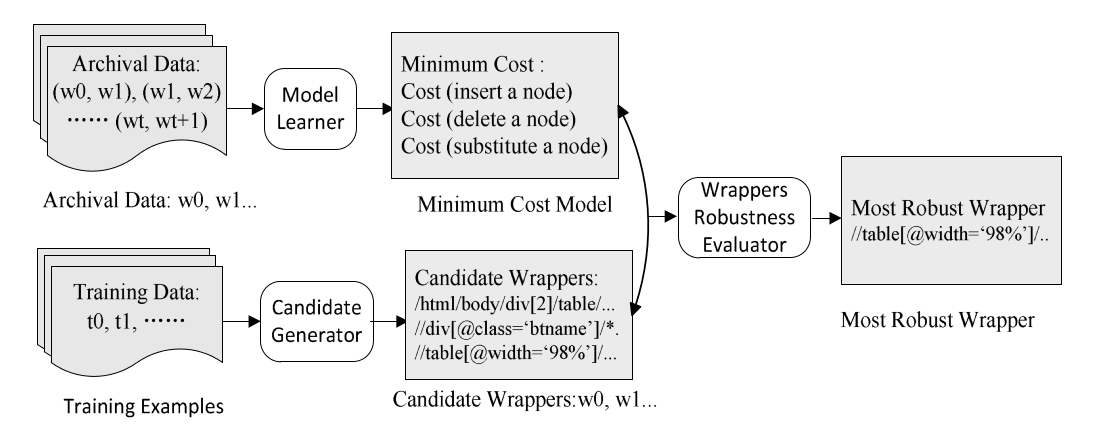
\includegraphics[width=\linewidth]{figures/robust-web-extraction-framework}


\section{Minimum Cost Edit Model}
% forther elaborate on the tool for the job

elaborate on the work so far:\\
- Zhang, Shasha\\
- A Survey on Tree Edit Distance and Related Problems\\
- RTED - A Robust Algorithm for the Tree Edit Distance\\
- Simple fast algorithms for the editing distance between trees and related problems\\
- React’s diff algorithm\\


\section{Generating candidate wrappers}


\section{Defining robustness}

- Optimal Schemes for Robust Web Extraction\\
- Robust Web Content Extraction\\
- Robust Web Extraction - An Approach Based on a Probabilistic Tree-Edit Model\\
- Robust Web Extraction Based on Minimum Cost Script Edit Model\\
- Robust Web Data Extraction - A Novel Approach Based on Minimum Cost Script Edit Model\\

% vim: set wrap
